\documentclass[12pt, oneside]{book}
\usepackage[a4paper,top=2.5cm,bottom=2.5cm,left=3.5cm,right=2cm]{geometry}


\ifx\uv\undefined\newcommand{\uv}[1]{,,#1``}\fi  

\renewcommand{\baselinestretch}{1.5}  % pre zvascenie riadkovania
\let\openright=\clearpage

%%%%% Nastavení kódování vstupních souborů: UTF-8
%%%%% ---------------------------------------------------------------
\usepackage[utf8]{inputenc} 
\usepackage[slovak,english]{babel}
\usepackage[T1]{fontenc}
\usepackage{lmodern}
\usepackage{minted}
\usepackage[babel=true]{microtype}

\usemintedstyle{tango}
\usepackage{lastpage}
\usepackage{lmodern}
\usepackage{amsmath}
\usepackage{amssymb,amsfonts,amscd}
\usepackage{array,hhline}
\usepackage{makeidx}
\usepackage{graphicx}
\usepackage{listings}
\usepackage{xcolor}
\usepackage{eurosym}
\usepackage{psfrag}
\usepackage{caption}
\usepackage{makecell}
\usepackage{graphicx}
\usepackage{subfig}
%%%%%%%%%%%%%%%%%%%%%%%%%%%%%%%%%%%%%%%%%%%%%%%%%%%%%%%%%%%%%%%%%%%%%%%%%%%%%%%%%%
%Define the listing package
\usepackage{listings} %code highlighter
\usepackage{color} %use color
\definecolor{mygreen}{rgb}{0,0.6,0}
\definecolor{mygray}{rgb}{0.5,0.5,0.5}
\definecolor{mymauve}{rgb}{0.58,0,0.82}
 
%Customize a bit the look
\lstset{ %
backgroundcolor=\color{white}, % choose the background color; you must add \usepackage{color} or \usepackage{xcolor}
basicstyle=\footnotesize, % the size of the fonts that are used for the code
breakatwhitespace=false, % sets if automatic breaks should only happen at whitespace
breaklines=true, % sets automatic line breaking
captionpos=b, % sets the caption-position to bottom
commentstyle=\color{mygreen}, % comment style
deletekeywords={...}, % if you want to delete keywords from the given language
escapeinside={\%*}{*)}, % if you want to add LaTeX within your code
extendedchars=true, % lets you use non-ASCII characters; for 8-bits encodings only, does not work with UTF-8
frame=single, % adds a frame around the code
keepspaces=true, % keeps spaces in text, useful for keeping indentation of code (possibly needs columns=flexible)
keywordstyle=\color{blue}, % keyword style
% language=Octave, % the language of the code
morekeywords={*,...}, % if you want to add more keywords to the set
numbers=left, % where to put the line-numbers; possible values are (none, left, right)
numbersep=5pt, % how far the line-numbers are from the code
numberstyle=\tiny\color{mygray}, % the style that is used for the line-numbers
rulecolor=\color{black}, % if not set, the frame-color may be changed on line-breaks within not-black text (e.g. comments (green here))
showspaces=false, % show spaces everywhere adding particular underscores; it overrides 'showstringspaces'
showstringspaces=false, % underline spaces within strings only
showtabs=false, % show tabs within strings adding particular underscores
stepnumber=1, % the step between two line-numbers. If it's 1, each line will be numbered
stringstyle=\color{mymauve}, % string literal style
tabsize=2, % sets default tabsize to 2 spaces
title=\lstname % show the filename of files included with \lstinputlisting; also try caption instead of title
}
%END of listing package%
 
\definecolor{darkgray}{rgb}{.4,.4,.4}
\definecolor{purple}{rgb}{0.65, 0.12, 0.82}
 
%define Javascript language
\lstdefinelanguage{JavaScript}{
keywords={typeof, new, true, false, catch, function, return, null, catch, switch, var, if, in, while, do, else, case, break},
keywordstyle=\color{blue}\bfseries,
ndkeywords={class, export, boolean, throw, implements, import, this},
ndkeywordstyle=\color{darkgray}\bfseries,
identifierstyle=\color{black},
sensitive=false,
comment=[l]{//},
morecomment=[s]{/*}{*/},
commentstyle=\color{purple}\ttfamily,
stringstyle=\color{red}\ttfamily,
morestring=[b]',
morestring=[b]"
}
 
\lstset{
language=JavaScript,
extendedchars=true,
basicstyle=\footnotesize\ttfamily,
showstringspaces=false,
showspaces=false,
numbers=left,
numberstyle=\footnotesize,
numbersep=9pt,
tabsize=2,
breaklines=true,
showtabs=false,
captionpos=b
}

%%%%%%%%%%%%%%%%%%%%%%%%%%%%%%%%%%%%%%%%%%%%%%%%%%%%%%%%%%%%%%%%%%%%%%%%%%%%%%%%%

\usepackage{url} 
\usepackage{bbding}         %%% balíček s nejrůznějšími
                            %%% symboly (čtverečky, hvězdičky,
                            %%% tužtičky, ručičky, nůžtičky, ...) 

\usepackage{paralist}       %%% lepší enumerate a itemize 
\usepackage{indentfirst}    %%% zaveď odsazení 1. odstavce
\usepackage[nottoc]{tocbibind} %%% zajistí přidání seznamu literatury,
                               %%% obrázků a tabulek do obsahu
\usepackage{tabularx}
\usepackage[pdftex,unicode,bookmarks=false]{hyperref}

\usepackage{fancyvrb}
\usepackage{fancyhdr} 
\fancyhf{}
\renewcommand{\headrulewidth}{0pt}
\cfoot{\thepage}

\usepackage{dirtytalk}
\usepackage{eurosym}

% \include{swift} % pridaný Swift highlighting

% Tato makra přesvědčují mírně ošklivým trikem LaTeX, aby hlavičky kapitol sázel příčetněji a nevynechával nad nimi spoustu místa. Směle ignorujte.
\makeatletter
\def\@makechapterhead#1{
  {\parindent \z@ \raggedright \normalfont
   \Huge\bfseries \thechapter. #1
   \par\nobreak
   \vskip 20\p@
}}
\def\@makeschapterhead#1{
 {\parindent \z@ \raggedright \normalfont
   \Huge\bfseries #1
   \par\nobreak
   \vskip 20\p@
}}
\makeatother

\newlength{\verbcorr}
\setlength{\verbcorr}{0ex}

\begin{document}

\selectlanguage{slovak}

\pagestyle{empty}
\pagenumbering{arabic}

%--------------------------------------------------------------------------------------
%%% hlavná stránka

\begin{titlepage}

\begin{center}

{\sc\LARGE Žilinská Univerzita v Žiline}

\medskip

{\sc\Large Fakulta riadenia a informatiky}

\vfill\vfill\vfill\vfill

{\sc\LARGE Bakalárska práca}

\smallskip

{\large Študijný odbor: {\bf Informatika}}

\end{center}

\vfill\vfill\vfill

\begin{center}
    
{\large\bf Jozef Chmelár}

\smallskip

{\large\bf Manažérsky systém pre správu projektov}

\smallskip

Vedúci: {\bf Ing. Viliam Tavač, PhD. }

\smallskip

Reg.č. 237/2015	

\smallskip

ŽILINA 2017

\end{center}

\end{titlepage}

%--------------------------------------------------------------------------------------
%%% cestne vyhlásenie

\pagebreak
\hfill
\vfill

\begin{center}

\sc\Large\textbf{Čestné vyhlásenie}

\end{center}

Čestne prehlasujem, že som prácu vypracoval samostatne s využitím dostupnej literatúry a vlastných vedomostí. Všetky zdroje použité v bakalárskej práci som uviedol v súlade s predpismi.

\vspace{1em}

Súhlasím so zverejnením práce a jej výsledkov.

\vspace{2em}

V Žiline, dňa 28.3.2017 \hfill ...........................

\hfill Jozef Chmelár \hspace{0,5em}

% \vfill
% \hfill
\pagebreak

%--------------------------------------------------------------------------------------
%%% poďakovanie

\pagebreak
\hfill
\vfill

\begin{center}

\sc\Large\textbf{Poďakovanie}

\end{center}

Týmto by som chcel poďakovať všetkým, ktorí mi pomohli pri vypracovaní bakalárskej práce. Ďakujem vedúcemu bakalárskej práce Ing. Viliam Tavač, PhD. za odbornú pomoc, pripomienky a usmerňovanie pri tvorbe práce.

\vspace{2em}

V Žiline, dňa 28.3.2017 \hfill ...........................

\hfill Jozef Chmelár \hspace{0,5em}

\pagebreak

%--------------------------------------------------------------------------------------
%%% slovensky abstrakt

\pagebreak

\begin{center}

\sc\Large\textbf{Abstrakt}
    
\end{center}

\noindent
{\sc CHMELÁR Jozef:} {\em Manažérsky systém pre správu projektov}
[Bakalárska práca] 

\noindent
Žilinská univerzita v Žiline,  
Fakulta riadenia a informatiky,  
Katedra softvérových technológií

\noindent  
Vedúci práce - Ing. Viliam Tavač, PhD. Stupeň odbornej kvalifikácie - Bakalár.- Žilina: FRI ŽU v Žiline, 2017 - Počet strán 42 
\noindent 



\vspace{1em}

Cieľom bakalárskej práce je navrhnúť a vytvoriť aplikáciu pre Android, zameranú na správu  projektov ktorá umožňuje efektívnejšiu komunikáciu medzi všetkými riešiteľmi projektu vo firme.

\vspace{1em}

\noindent
{\bf Kľúčové slová:} Android, aplikácia, projekt manažment

\pagebreak

%--------------------------------------------------------------------------------------
%%% anglicky abstrakt

\selectlanguage{english}

\pagebreak

\begin{center}

\sc\Large\textbf{Abstract}
    
\end{center}

\noindent
{\sc CHMELÁR Jozef:} {\em Project's manager system for project manager
}
[Bachelor thesis] 

\noindent
University of Žilina,  
Faculty of Management Science and Informatics,  
Department of Software Technologies

\noindent  
Supervisor: Ing. Viliam Tavač, PhD.  - Qualification level : Bachelor.- Žilina: FRI ŽU in Žilina ,2017 - Number of pages: 42 


\vspace{1em}

Goal of the bachelor thesis is to design and create Android application which will provide a more efficient  way to communicate between all collaborators of projects within a company.

\vspace{1em}

\noindent
{\bf Keywords:} Android, application, project management

\pagebreak

\selectlanguage{slovak}

\pagestyle{myheadings}

\setcounter{page}{7}

%%%%%%%%%%%%%%%%%% obsah

{
\setlength{\parskip}{1pt plus 1pt}

\markboth{}{}

\pagestyle{fancy}

% obsah
\tableofcontents

% zoznam obrazkov
\listoffigures

% zoznam tabuliek
\listoftables

% zoznam skratiek
\chapter*{Zoznam skratiek a termínov}
\addcontentsline{toc}{chapter}{Zoznam skratiek a termínov}

\begin{tabularx}{\textwidth}{@{}>{\bfseries\raggedright\hsize=.4\hsize}X >{\hsize=1.6\hsize}X@{}}
        
        \textbf{AOKP} & Android Open Kang Project \label{AOKP}\\
    \textbf{AOSP} & Android Open Source Project \label{AOSP}\\
    \textbf{API} & Application programming interface \label{api}\\
    \textbf{APK} & Android package \label{apk}\\
    \textbf{ART} & Android Runtime Enviroment  \label{art}\\
    \textbf{GUI} & Graphical User Interface \label{gui}\\
    \textbf{JDK} & Java Development Kit \label{jdk}\\
    \textbf{JRE} & Java Runtime Enviroment  \label{jre}\\
    \textbf{JSON} & JavaScript Object Notation \label{json}\\
    \textbf{JVM} & Java Virtual Machine  \label{jvm}\\
    \textbf{JWT} & JSON Web Token   \label{jwt}\\
    \textbf{MIUI} & Mi User Interface\label{api}\\
    \textbf{MVP} & Model, View, Presenter \label{mvp}\\
    \textbf{ORM} & Object-relational mapping \label{orm}\\
    \textbf{PaaS} & Platform as a service  \label{PaaS}\\
    \textbf{REST} & Representational state transfer  \label{rest}\\
    \textbf{SDK} & Software Development Kit - Súbor nástrojov pre vývoj softvéru \label{sdk}\\
    \textbf{SSH} & Kryptovaný sieťový protokol \label{sdk}\\
    \textbf{URL} & Jednotný vyhľadávač prostriedku \label{sdk}\\
    \textbf{XML} & eXtensible Markup Language \label{xml}\\

 \end{tabularx}
}

\markboth{}{}

\clearpage

%%%%%%%%%%%%%%%%%% obsah - koniec

\pagestyle{fancy}

%%%%%%%%%%%%%%%%%% kapitoly

\chapter*{Úvod}
\addcontentsline{toc}{chapter}{Úvod}

Žijeme v dobe kedy výkonné mobilné zariadenia nepatria medzi majetok vyvolených ľudí, ale takmer o samozrejmú výbavu každého človeka, či už sa jedná o študenta, alebo prezidenta. Je úžasné a zároveň úsmevné ako namiesto obyčajného budíka používame zariadenie s porovnateľným výkonom ako počítač z pred pár rokov. Veľa ľudí pred spánkom zapojí svoj telefón do nabíjačky, ráno ich zobudí a sprevádza ho celý deň. Objekty reálneho sveta ako poznámkový blok, telefónny zoznam, mapa, fotoaparát alebo prehrávač hudby nahradili rovnomenné aplikácie a všetky sa zmestia do vrecka nohavíc. 

Počas pobytu v rýchlo rastúcej spoločnosti kde nie každý pracovník firmy mal prístup k počítaču, rôzne oddelenia mali vlastné systémy na internú komunikáciu, pričom neraz to bol obyčajný email, ale s rastom spoločnosti prestali dostačovať, a videl som potenciál práve na zariadeniach ktoré má väčšina zamestnancov, ich inštalácia a nasadzovanie netrvá mesiace, ale minúty. Rovnako som chcel zabezpečiť jednoduchý kontakt na rôznych riešiteľov projektov, keďže  veľa ľudí na seba navzájom nemala kontakt, prístup na server k excel tabuľke s kontaktmi, o ktorej existencii viacerí zamestnanci ani nevedeli. 


\vspace{10pt}
Táto práca sa zaoberá vytvorením mobilnej aplikácie pre Android, ktorá používa najznámejšie technológie v oblasti mobilného vývoja a umožní uľahčenie komunikácie medzi zamestnancami, ktorí nemajú svoj pracovný počítač, ale ich prácu by uľahčilo a zrýchlilo práve zariadenie, ktoré dávno majú.      % Úvod
\chapter{Súčasný stav}

Android je operačný systém ktorý je založený na licencii open source\cite{android}. To znamená, že hocikto môže bezplatne sťahovať a distribuovať jeho zdrojový kód. To dospelo do súčasného stavu, kedy má prístup k výkonným mobilným zariadeniam väčšia časť populácie ako kedykoľvek predtým. Každá spoločnosť si môže upraviť Android podľa vlastných predstáv a poskytnúť zákazníkovi jedinečné prostredie. Okrem toho získali vývojári prístup k veľkému publiku, keďže vývojári nemuseli platiť za licencie, alebo vyvíjať vlastný operačný systém. To umožnilo vývojárom znížiť náklady na vývoj a od roku 2011 do 2013 klesla priemerná cena smartphonov na celom svete o 25\% \cite{cena_smartphone}. Pokiaľ by sme chceli stráviť jednu minútu prezeraním každého jedného zariadenia s Androidom, trvalo by nám to dva a pol týždňa bez spánku. Momentálne existuje na svete 24000 zariadení od takmer 1300 značiek \cite{pocetTelefonov}. Vďaka Androidu vznikli rôzne verzie, medzi ktoré patrí CyanogenMod, MIUI, AOKP momentálne je najpoužívanejšia verzia Androidu je 5.0-5.1 Lollipop s 32,5\% podielom na trhu \cite{usage}, ostatné verzie a ich podiel na trhu môžeme vidieť na grafe (obr.\ref{obr1.1}.)

\begin{figure}[ht]
    \begin{center}
        \begin{minipage}{0.99\linewidth}
            \begin{center}
                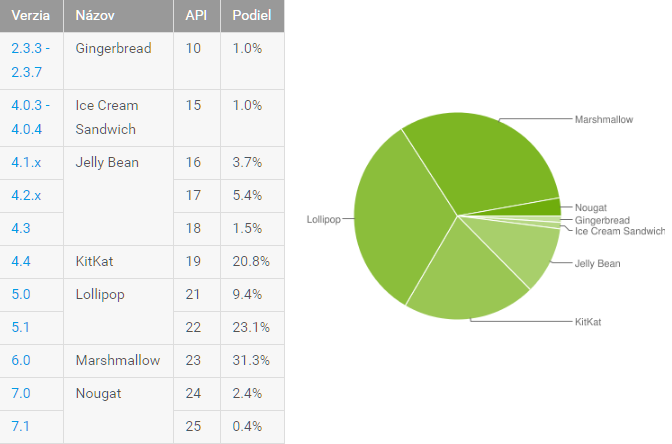
\includegraphics[width=0.99\textwidth]{images/verzie_and.png}
                \caption{Podiel verzií Androidu}
                \label{obr1.1}
            \end{center}
        \end{minipage}
    \end{center}
\end{figure}
 

Ponuka, ktorú nám Android prináša, nekončí pri počte zariadení, ale aj aplikáciami, ktorých je cez Google Play dostupných viac ako 1 milión \cite{android}. Dostupné sú aj alternatívy ku Google a to Amazon Appstore, GetJar, Mobogenie, SlideME, F-Droid \cite{playstore_alt}.

\section{História}

Spoločnosť Android Inc. bola založená v Palo Alto, California v Októbri 2003 \cite{history_android}.Pri vzniku stáli Andy Rubin, Rich Miner, Nick Sears a Chris Whie s myšlienkou vytvoriť múdrejšie mobilné zariadenia, ktoré by si boli vedomé o svojej pozícii a používateľových preferenciách. Pôvodný úmysel spoločnosti bol vyvinúť pokročilý operačný systém pre digitálne fotoaparáty,ale  malý trh ich naviedol na cestu vývoja pre mobilné zariadenia a konkurovať tak Symbianu a Windows Mobile. \cite{history_cameras}


\section{Verzie Androidu}
Najvyššie číslo dostupnej verzie operačného systému Android je \textit{7.0} a vzhľadom k tomu sa už staršie verzie vo veľkom počte nepoužívajú, preto sa budeme v nasledujúcich podkapitolách venovať len verziám s minimálnym podielom 15\%

\begin{description}
\item[KitKat] Vydaný v Októbri 2013 bol vylepšený oproti predošlým verziám  o nástroj na analýzu pamäte, nahrávanie obrazovky, API k infračervenému blastru a audio monitoring. Od tejto verzie majú vývojári prístup k SMS API. \cite{versions} . Dalšie podverzie 4.4.1 až 4.4.4 priniesli hlavne bezpečnostné opravy.


\item[Lollipop] Najväčšiu zmenu, ktorú Lollipop priniesol ku koncu roka 2014 do androidu  bol nový dizajn používateľského prostredia vybudovaný pomocou dizajnového jazyka \textit{Material Design} ktorý je hlavným vizuálnym prvkom Googlu. Virtuálny stroj Dalvik bol nahradený Android Runtime\cite{dalvik}. Lollipop 5.0.1 - 5.1.1, pridali podporu viacerých SIM a  ochranu zariadenia pri krádeži.


\item[Marshmallow] Pribudol správca povolení pre aplikácie. API ,ktoré umožňuje pristupovať k práve zobrazeným dátam na obrazovke. Od 6.0 Android natívne podporuje odtlačky prstov a USB-C a funkcia \textit{deep sleep}, ktorá pomáha šetriť batériu v prípade potreby.


\item[Nougat] Predstavil výrazné zmeny. Pribudla možnosť zobraziť viaceré aplikácie na jednej obrazovke, rozdelenie obrazovky na časti, instantné odpovede priamo v notifikačnom centre a optimalizačné prvky pre virtuálnu realitu.

\end{description}

\chapter{Použité technológie}

Operačný systém Android je naprogramovaný hlavne v jazyku Java \cite{android_code}  (tab. \ref{tab:android_code}), rovnako ako aj aplikácie. Pre vývoj je potrebné mať nainštalované JDK spolu s  SDK Manager, pomocou ktorého môžeme stiahnuť potrebné verzie Android SDK, obsahujúce nástroje , ktoré kompilujú kód spolu s inými časťami aplikácie ako sú obrázky, jazykové súbory do APK archívu , ktorý obsahuje všetky súbory potrebné na inštaláciu. Android je multi-user Linux systém, v ktorom je každá aplikácia definovaná ako používateľ. Každá aplikácia má priradené unikátne používateľské ID pomocou ktorého systém obmedzí povolenia pre aplikáciu.Každá aplikácia má svoj Linux proces, ktorý je vytvorený vždy. keď je potrebné spustiť komponent aplikácie, a je ukončený vždy keď proces nie je naďalej potrebný alebo systém potrebuje pamäť pre iné aplikácie.


\vspace{10pt}

\begin{table}[hb!]
    \centering
    \begin{tabular}{| l | l | }
    \hline
        Jazyk   &   Podiel kódu     \\  \hline
        Java    &   46,1\%          \\  \hline
        C       &   30,8\%          \\  \hline
        C++     &   13,4\%          \\  \hline
        Ostatné &   9,7\%           \\  \hline
    \end{tabular}
    \caption{Percentuálny podiel jazykov v AOSP}
    \label{tab:android_code}
\end{table}

\section{Nástroje}

Vývoj softvéru sa nezaobíde bez výberu správnych nástrojov. Nie sme nútení písať aplikácie v obyčajných textových editoroch, máme k dispozícií veľké množstvo prepracovaných vývojových nástrojov ktoré umožňujú rýchly re-faktoring kódu, analýzu kódu, build systémy pre ľahší a rýchlejší vývoj. Za nástroje považujeme aj súčasné technológie, ktoré uľahčujú prácu s rôznymi časťami aplikácie a poskytujú nám abstrakciu, ktorá umožní písať kvalitný a čitateľný kód.

\section{Android Studio}

Od 26.Júna.2015 prestal Google oficiálne vyvíjať plugin pre IDE Eclipse \cite{androidstudio} a Android Studio sa stalo jediným oficiálne podporovaným nástrojom na vývoj pre platformu Android. Na jeho vývoji sa podieľa Google a taktiež spoločnosť JetBrains ktorá vyvíja IntelliJ Idea, na ktorom je Android Studio založené. Medzi jeho výhody patria \cite{androidstudio2} 


\begin{itemize}

\item Build nástroj Gradle, ktorý automaticky zostavuje aplikáciu spolu s knižnicami, alebo inými projektami
\item Refaktoring špecifický pre Android
\item ProGuard ktorý zmenšuje veľkosť aplikácie, maže zbytočný kód a komplikuje reverzné inžinierstvo
\item Android špecifické šablóny
\item GUI editor 
\item Hĺbková analýza kódu

\end{itemize}

\section{IntelliJ Idea}

Android Studio a Android plugin pre IntelliJ Idea sú postavené na rovnakom kóde \cite{androidstudio3} pričom nedostaneme pred-konfigurovaný nástroj na vývoj priamo od inštalácie. Jedná sa o produkt, ktorý je primárne IDE pre Javu a J2EE. Projekty, vytvorené v Android Studio, je možné otvoriť v IntelliJ Idea a vice versa. Spoločnosť JetBrains poskytuje pluginy ktoré poskytujú lepšiu prácu s verzionovacím systémom alebo databázou.


\section{Kotlin}

Kotlin je staticky typovaný jazyk bežiaci nad JVM vyvíjaný \textit{JetBrains}, ktorý síce nie je syntakticky kompatibilný s Javou, ale je navrhnutý tak, že umožňuje využívať všetky Java knižnice. Narozdiel od  Javy si nevyžaduje veľa písania, podporuje lambda výrazy, dátové triedy a automaticky generuje metódy na prístup k premenným. Jedná sa o čoraz viac využívaný jazyk Android  vývojármi \cite{kotlin}. 

\section{ReactiveX}

Reactive Extensions (Rx) je knižnica na vytváranie asynchrónnych udalostne založených programoch. Uľahčuje prácu pri súbežných výpočtoch a poskytuje abstrakciu, ktorá nás odbremení najmä od synchronizácií vlákien. Rx je založený na návrhovom vzore Pozorovateľ - Vydavateľ

\begin{figure}[H]
    \begin{center}
        \begin{minipage}{0.9\linewidth}
            \begin{center}
                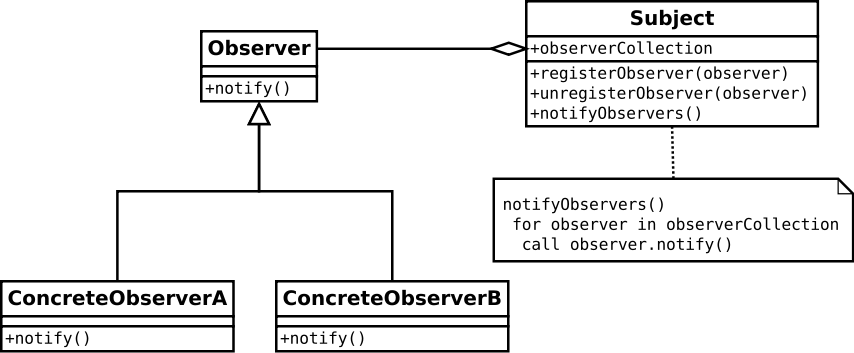
\includegraphics[width=0.9\textwidth]{images/rx.png}
                \caption{Pozorovateľ - Vydavateľ - bdiagram tried }
                \label{obr2.1}
            \end{center}
        \end{minipage}
    \end{center}
\end{figure}

Vždy ak vydavateľ zmení hodnotu, všetci pozorovatelia budú upozornení, čo je užitočné hlavne pri zobrazovaní informácií pre používateľa, každá zmena v premennej môže byť automaticky zobrazená používateľovi. Pri Http požiadavke môžeme na jednom vlákne sledovať stav požiadavky, pokiaľ požiadavka skončí, či už chybou alebo úspešne, sme schopní zobraziť informáciu používateľovi okamžite na UI vlákne.

\section{Cloudové služby}

Väčšina aplikácií komunikuje so vzdialeným serverom, ktorý odpovedá na požiadavky klienta. Nastavovanie serverovej časti aplikácie, inštalácia potrebného softvéru  a následná údržba stojí čas , ktorý je pri tvore softvéru veľmi vzácny, preto sa na trhu začali objavovať PaaS služby ktoré, vývojárovi ušetria čas.

\subsection{Heroku}
Heroku je jedna z prvých cloudových platforiem, ktorá je vyvíjaná od roku 2007. Vtedy podporovala nasadenie aplikácií len v jazyku Ruby, dnes podporuje  Javu, Node.js, Scala, Clojure, Python, PHP, a Go. Heroku poskytuje jednoduché nasadenie aplikácie priamo z verzionovacieho systému Git, ktorý poskytuje prehľad všetkých zmien v kóde. Heroku poskytuje vlastný Git repozitár, alebo napojenie na GitHub, pričom pri aktualizácii hlavnej vetvy repozitáru sa aplikácia sama skompiluje a nainštaluje. \cite{heroku}

\subsection{OpenShift}
OpenShift je PaaS produkt za ktorým stojí spoločnosť RedHat, ktorá poskystuje hosting s vývojársky prívetivými službami ako MongoDB, Node.js prístup cez webové rozhranie alebo príkazový riadok. Obsahuje všetky závislosti, potrebné na vývoj  Java Enterprise aplikácií, integráciu s IDE a automatizačnými systémami ako Maven alebo Jenkins. OpenShift dbá na zabezpečenie, preto je možné komunikovať len pomocou SSH kľúča. Rovnako ako na Heroku, aplikácia sa builduje z Git repozitáru. 

\chapter{Analýza}

\section{Klient-server} 
Architektúra klient server rozdeľuje aplikáciu na dve časti. Serverová aplikácia, ktorá je spustená na výkonnom zariadení spracováva dáta, poskytuje veľkú pamäť, alebo databázu a klientskú časť, ktorá poskytuje používateľské prostredie na odosielanie požiadaviek a zobrazenie odpovede servera\cite{clientserver}. Android aplikácie najčastejšie používajú REST architektúru, ktorá využíva URL adresu a HTTP požiadavky na interakciu so serverom. 

\begin{table}[H]
\centering
\caption{REST komunikácia}
\label{REST komun}
\begin{tabular}{|l|l|l|}
\hline
\textit{URL/Http Metóda}             & \multicolumn{1}{c|}{\textit{\textbf{GET}}} & \multicolumn{1}{c|}{\textit{\textbf{PUT}}} \\ \hline
\textit{\textbf{uniza.sk/student}}   & Vráti kolekciu študentov                   & Nahradí kolekciu novou                     \\ \hline
\textit{\textbf{uniza.sk/student/1}} & Zobrazí informácie o študentovi s id 1     & Nahradí staré údaje novými                 \\ \hline
\textit{URL/Http Metóda}             & \multicolumn{1}{c|}{\textbf{POST}}         & \multicolumn{1}{c|}{\textbf{DELETE}}       \\ \hline
\textit{\textbf{uniza.sk/student/1}} & Vytvorí novú položku a vráti jej URI       & Vymaže kolekciu                            \\ \hline
\textit{\textbf{uniza.sk/student/1}} & Vo všeobecnosti sa nepoužíva.              & Vymaže študenta z kolekcie                 \\ \hline
\end{tabular}
\end{table}

Klient posiela požiadavky na server buď pomocou URL adresy alebo s dodatočnými dátami uložené v tele požiadavky vo formáte Json, alebo XML.

\section{Základné komponenty aplikácie}
Všetky prvky operačného systému sú prístupne pre programátora pomocou API, ktoré sú naprogramované v jazyku Java. Všetky prvky tvoria stavebné bloky, ktoré potrebujeme na vývoj aplikácie. Sú to znova použiteľné a modulárne komponenty.
\subsection{Aktivita}
 
Aktivita reprezentuje jednu obrazovku, ktorá obsahuje všetky komponenty nutné pre interakciu s aplikáciou. Aktivity sú v systéme  spravované ako zásobník aktivít, nová aktivita je vždy pridaná na vrchol zásobníka, pričom predošlé aktivity ostávajú v zásobníku a nebudú zobrazené kým neodídeme z vrchnej aktivity.
Aktivita má štyri stavy. Pokiaľ je aktivita zobrazená na obrazovke je aktívna, alebo bežiaca. Ak aktivitu prekryje iné okno, ale je stále viditeľná tak je pozastavená, čo znamená, že celý jej stav je uložený a je stále aktívna. Ak je aktivita celá prekrytá novou, pôvodná je zastavená. Hoci si o sebe uchováva všetky informácie, nie je používateľovi viditeľná a môže byť kedykoľvek zmazaná z pamäte, ak systém potrebuje pamäť na inom mieste.
Nasledujúci diagram  (obr.\ref{obr1.2}.) zobrazuje životný cyklus aktivity.

\begin{figure}[H]
    \begin{center}
        \begin{minipage}{0.80\linewidth}
            \begin{center}
                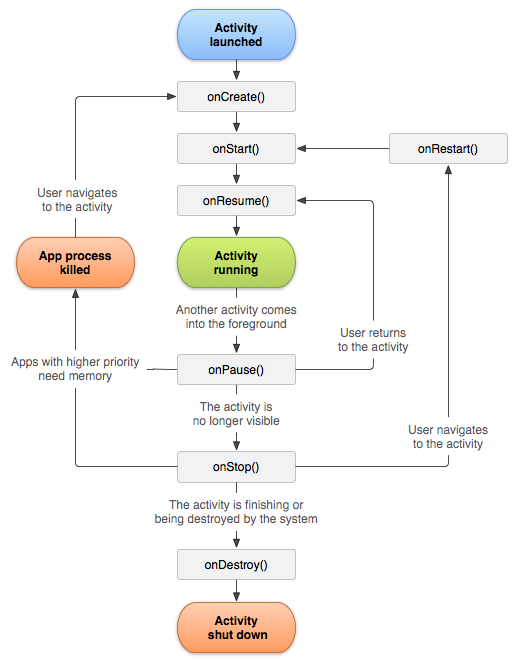
\includegraphics[width=0.85\textwidth]{images/activity_lifecycle.png}
                \caption{Životný cyklus aktivity}
                \label{obr1.2}
            \end{center}
        \end{minipage}
    \end{center}
\end{figure}

\subsection{Služba}
Service, alebo služba, je aplikačný komponent, ktorý umožňuje vykonávať dlhotrvajúce činnosti na pozadí ako je napríklad prehrávanie hudby alebo získavanie dát z GPS. Služba je spustená aplikáciou a ostáva spustená aj po jej ukončení. Má jednoduchý životný cyklus. Aplikácia ju spustí a beží až kým nie je zastavená operačným systémom, alebo spúšťajúcou aplikáciou \ref{obr1.3}.

\begin{figure}[H]
    \begin{center}
        \begin{minipage}{0.5\linewidth}
            \begin{center}
                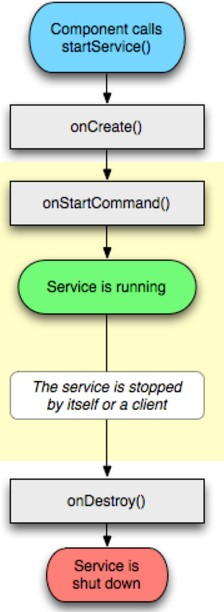
\includegraphics[width=0.5\textwidth]{images/service_life.jpg}
                \caption{Životný cyklus služby}
                \label{obr1.3}
            \end{center}
        \end{minipage}
    \end{center}
\end{figure}

\subsection{Poskytovateľ obsahu}
Poskytovateľ obsahuje spravuje dáta, ktoré môžu byť zdieľanie napriek aplikáciami pomocou  SQLite databázy. Ak má aplikácia práva, môže meniť obsah dát, ktoré sú dostupné, následne iná aplikácia dostane po vyžiadaní dát, nové a upravené hodnoty. Príklad využitia takejto služby je telefónny zoznam, kedy môže aplikácia tretej strany pristupovať k číslam, využívať ich, prípadne meniť.

 
\section{Aktuálne riešenia}
Cieľom tejto analýzy je porovnať dostupnosť, jednoduchosť a cenu súčasných najpoužívanejších riešení, ktoré sú dostupné na trhu.

  \vspace{10pt}
\subsection{JIRA Software}


\textit{JIRA Software} od spoločnosti Atlassian je software na správu projektov pre agilné tímy. Pomocou takzvaných Kanban boardov, ktoré umožňujú celému tímu vidieť aká práca ich v najbližšom období čaká, momentálne prebieha alebo je už dokončená. Jedná sa o tabuľku s kartičkami s obsahom práce, ktoré môžu následne členovia tímu premiestňovať do adekvátnych stĺpcov (obr.\ref{obr2.1}.)



\begin{figure}[ht]
    \begin{center}
        \begin{minipage}{0.99\linewidth}
            \begin{center}
                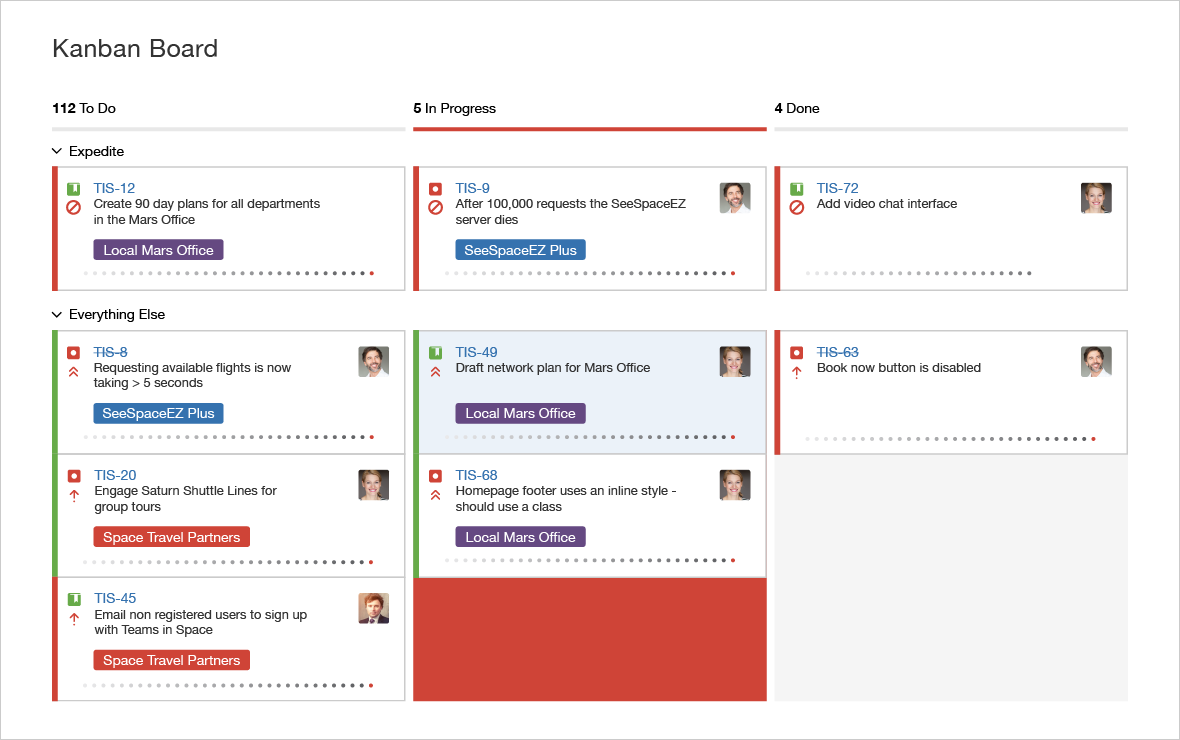
\includegraphics[width=0.99\textwidth]{images/kanbanboard.png}
                \caption{Kanban board}
                \label{obr2.1}
            \end{center}
        \end{minipage}
    \end{center}
\end{figure}

\vspace{10pt}

Každá kartička v tabuľke reprezentuje úlohu, ktorá má vždy zadávateľa a osobu, ktorá bude danú úlohu vykonávať a následne aktualizovať jej stav. Pri vytvorení a priradení úlohy príde riešiteľovi emailové oznámenie o priradení. Jedná sa o relatívne zdĺhavý proces, ktorý zamestnanci neradi vykonávajú. JIRA software je o mnoho obsiahlejší, tým pádom komplikovanejší, a napriek user-friendly prostrediu vyžaduje zaškolenie nového zamestnanca a firmy potrebujú vlastného JIRA správcu. Jedná sa ale o najobľúbenejšie riešenie pre projektový manažment ktorý umožňuje firmám lepšiu organizáciu pri riadení práce, ktorého výsledkom je kvalitný finálny produkt dodaný načas. Taktiež je rožsíriteľný o dalšie produkty spoločnosti ako sú Confluence, Bitbucket, Trello. Chýba im ale dedikovaná, jednoducha a funkčná aplikácia pre mobilné telefóny

Atlassian ponúka tri verzie ich softvéru. Verzia, ktorá sa nainštaluje na vlastný server, verzia v data centre a cloudová inštancia ich produktu. Základná verzia JIRA Core pre 25 ľudí stojí  \$1800 za serverovú aplikáciu a \$180 mesačne za cloudovú inštanciu .

\vspace{10pt}

\subsection{Slack}

\textit{Slack} je nástroj na tímovú kolaboráciu, ktorý vznikol ako interný nástroj, a v súčasnej dobe sa jedná o cloudovú službu. Jedná sa v podstate o interný chat, ktorý je rozdelený do rôznych kanálov. Kanál  (obr.\ref{obr2.2}) reprezentuje tému, projekt, lokácie alebo skupinu ľudí.


Ľudia môžu pomocou Slack-u posielať správy aj konkrétnej osobe, uskutočňovať hovory, zdieľať súbory. Externé firmy, ktoré taktiež využívajú Slack, môžu využívať spoločný kanál. Najväčšou výhodou Slack-u je, že odpadáva nutnosť odosielať hromadné maily, v ktorých sa po čase stráca prehľad, sprehľadňuje email a prenecháva mu jeho dôležitú funkciu a to  komunikáciu s  dôležitými klientmi pre formálnejší spôsob posielania správ. 
Na rozdiel od JIRA Software je Slack dostupný len z cloudu, na ktorý sa možno pripojiť cez webový prehliadač alebo aplikáciou pre všetky desktopové a mobilné platformy, pričom sa jedná o stabilné a prepracované produkty. Ponúka verziu zadarmo, ktorá ale na rozdiel od platených,  neposkytuje šifrovanie, externý prístup pre klientov alebo video konferencie.


\begin{figure}[H]
    \begin{center}
        \begin{minipage}{0.95\linewidth}
            \begin{center}
                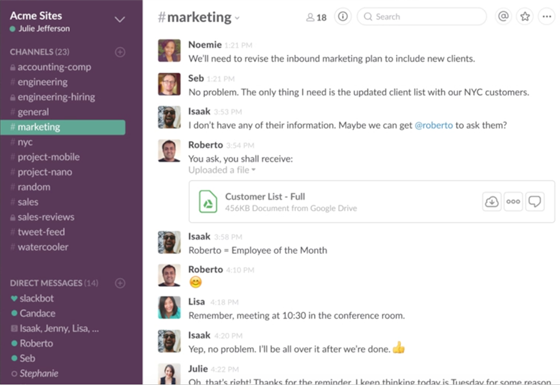
\includegraphics[width=0.99\textwidth]{images/slack.png}
                \caption{Slack, hlavné okno}
                \label{obr2.2}
            \end{center}
        \end{minipage}
    \end{center}
\end{figure}
 
\vspace{10pt}
Jedná sa o veľmi obľúbený nástroj, ktorý plní viac úlohu rýchleho chatu medzi kolegami v práci, ktorí niečo rýchlo potrebujú, ale nie sú dostatočne urgentné na telefonický rozhovor alebo posielanie mailu. 
 


\vspace{10pt}

Cieľom a úlohou tejto práce bolo navrhnúť a vytvoriť aplikáciu, ktorá by zahŕňala výhody predchádzajúcich riešení a v spojení so zadaním by bola vo finále ideálnym riešením pre malý a stredný podnik.
  
  
\section{Zber požiadaviek}

Aplikácia má poskytnúť jednoduché a intuitívne používateľské prostredie, ktoré dovolí používateľovi vidieť na akých projektoch pracuje, správy ktoré si riešitelia poslali, zapisovanie služobných ciest a jednoduchú komunikáciu medzi používateľmi. 

\begin{figure}[H]
    \begin{center}
        \begin{minipage}{0.9\linewidth}
            \begin{center}
                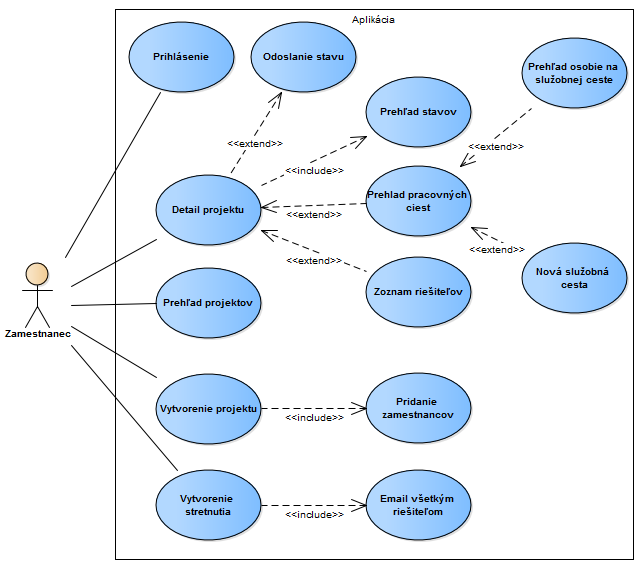
\includegraphics[width=0.9\textwidth]{images/usecase.png}
                \caption{Prípady použitia }
                \label{obr2.1}
            \end{center}
        \end{minipage}
    \end{center}
\end{figure}

Projekt by mal obsahovať všetkých ľudí ktorí na ňom pracujú, ich telefónne čísla, email a pracovnú pozíciu. Organizácia pracovného stretnutia je oznámená všetkým riešiteľom s dátumom a miestom konania na ich emailové adresy. 




\chapter{Návrh a implementácia aplikácie}

Aby aplikácia podporovala čo najväčšie množstvo zariadení, bude minimálna podporovaná verzia Androidu 4.4, a kedže sa jedná a natívne vyvíjanú aplikáciu, použijeme oficiálny nástroj Android Studio.  Za programovací jazyk bola zvolená kombinácia Javy a Kotlinu, keďže sú podporované zvoleným IDE od inštalácie a majú veľkú komunitu spolu s množstvom knižníc. Serverovú časť aplikácie má na starosti služba Heroku, na ktorej je nasadená Node.JS aplikácia, ktorá sa správa ako most medzi MongoDB databázou ktorú poskytuje služba mlab.com \ref{obr3.4}. Na rozdiel od Slacku a JIRA, táto aplikácie ponúkne minimalistické používateľské prostredie a jednoduchosť. V návrhu popíšeme klientskú aj serverovú časť architektúry aplikácie.


\vspace{10pt}
\begin{figure}[H]
    \begin{center}
        \begin{minipage}{0.9\linewidth}
            \begin{center}
                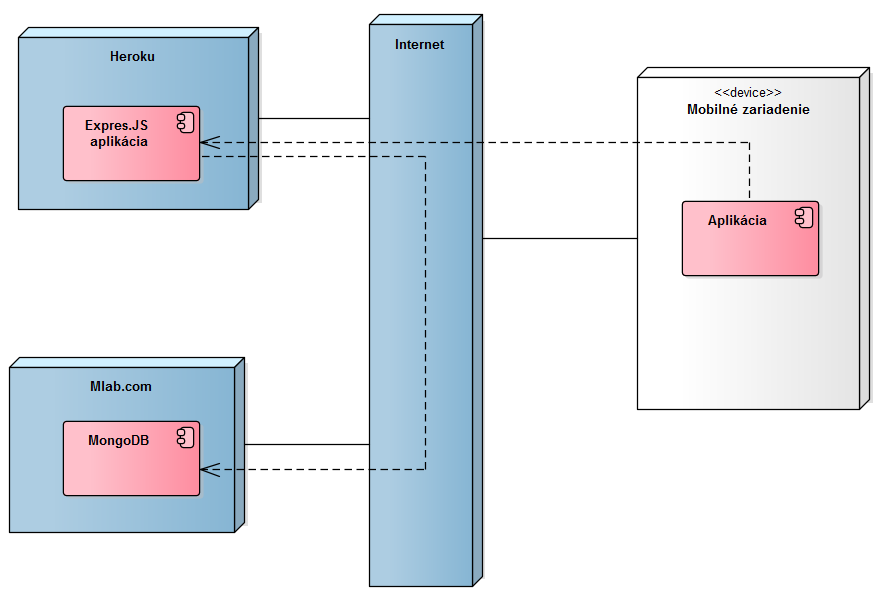
\includegraphics[width=0.9\textwidth]{images/deploy.png}
                \caption{Diagram nasadenia}
                \label{obr3.4}
            \end{center}
        \end{minipage}
    \end{center}
\end{figure}
\vspace{10pt}



\section{Architektúra aplikácie}
Pri návrhu aplikácie sme sa držali princípu oddelenia zodpovedností. Aby bol kód ľahšie rozšíriteľný a v budúcnosti znova použiteľný rozhodli sme sa pre našu aplikáciu aplikovať architektonický vzor
Model-View-Presenter. 
\vspace{10pt}
\begin{figure}[H]
    \begin{center}
        \begin{minipage}{0.9\linewidth}
            \begin{center}
                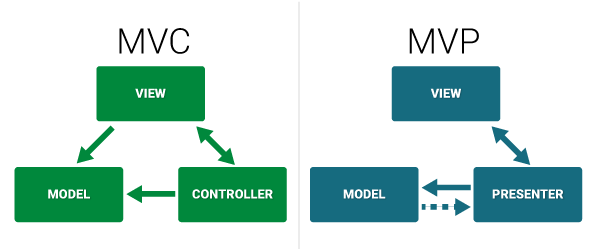
\includegraphics[width=0.9\textwidth]{images/MVC_MVP.png}
                \caption{Porovnanie MVP s MVC }
                \label{obr3.1}
            \end{center}
        \end{minipage}
    \end{center}
\end{figure}
\vspace{10pt}

Vzor nám umožní kompletne oddeliť biznis logiku od používateľského prostredia a to rozdelením ich zodpovedností \cite{mvpdef}.

\begin{description}
\item[Presenter]
 plní úlohu mostu medzi View a Modelom. Získava dáta z modelu a naformátované ich presúva do View modulu. Na rozdiel od MVC, rozhoduje aj o tom čo sa stane, keď nastane akcia vo view. 

\item[View]
 je implementovaný ako aktivita, ktorá si uchováva referenciu na presenter. Jediná vec ktorú view robí, je že volá metódy presentera.

\item[Model]
 v našej aplikácii predstavuje reprezentáciu dát, ktoré sú uložené v databáze, a aj s ňou komunikuje.

\end{description}

Aplikovanie vzoru (obr.\ref{obr3.1}) na Android je jednoduché. Vytvoríme rozhranie \textit{IView}   (obr.\ref{obr3.2}) ktoré reprezentuje všetky používateľské akcie, ako napríklad zobrazenie animácie, oznámenie o dokončení požiadavky na server a pod.

\vspace{10pt}
\begin{figure}[H]
    \begin{center}
        \begin{minipage}{0.9\linewidth}
            \begin{center}
                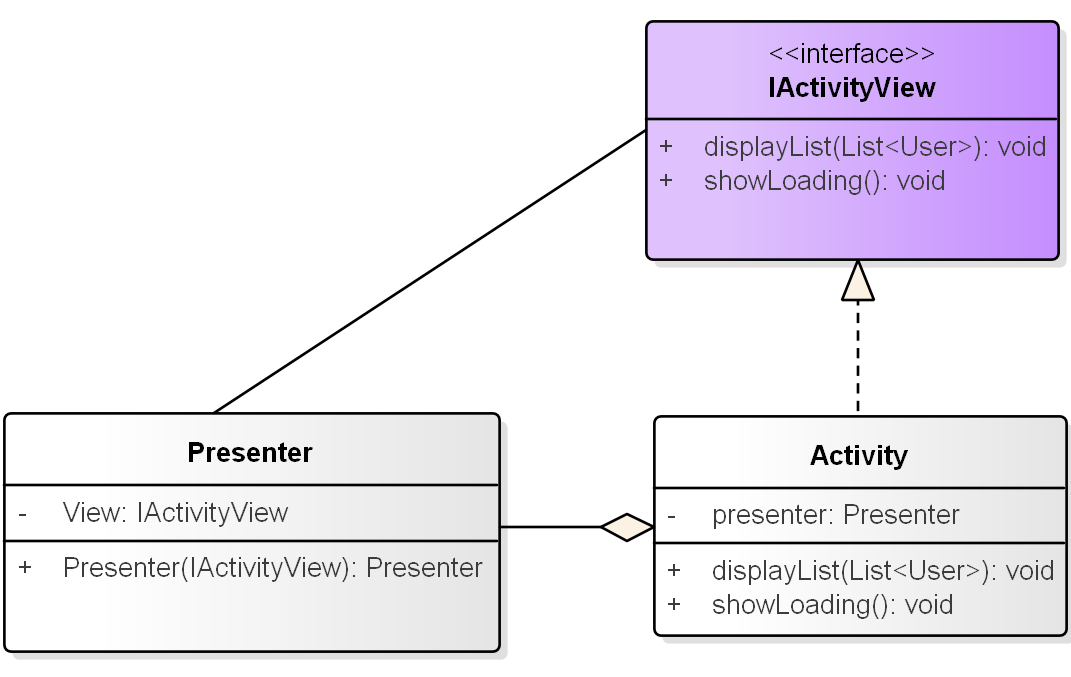
\includegraphics[width=0.9\textwidth]{images/mvpandroid.png}
                \caption{Nasadenie MVP v Androide }
                \label{obr3.2}
            \end{center}
        \end{minipage}
    \end{center}
\end{figure}
\vspace{10pt}

Presenter obsahuje objekt rozhrania, ktorý je aj parametrom konštruktora. Následne môže presenter volať metódy rozhrania. View implementuje rozhranie a všetky jeho metódy. V nich následne implementujeme kód, ktorý súvisí s View, ako je komunikácia s komponentami Androidu ako sú ListView, Progressbar a iné. Takýmto spôsobom oddelíme kód ktorý súvisí s Androidom od našej logiky, tým pádom presenter obsahuje kód, nezávislý na platforme na ktorý je možné napísať unit testy.

Aplikácia obsahuje triedu \textit{App}, ktorá je potomkom triedy \textit{Application}, ktorej inštancia je vytvorená skôr, ako ktorákoľvek iná trieda v balíčku aplikácie. To využívame na vytvorenie objektu klienta na komunikáciu s REST API, ktorý následne vkladáme do presentera aktivity, ktorá využíva sieťovú komunikáciu. Vytvorenie viacerých inštancií Http klienta by bolo zbytočné, keďže sa skladá z obsiahlych knižníc ako serializér a deserializér JSON objektov \textit{GSON}, Http knižnice \textit{OkHttp} a \textit{Retrofit}, ktorý uľahčuje prácu s REST API.

\section{Prihlasovacia obrazovka}

Prihlasovacia obrazovka slúži ako vstupná brána do aplikácie. Obsahuje polia pre email a heslo a tlačidlá prihlásenie, registráciu. Pri nesprávnom formáte emailu ktoré overuje regulárny výraz, alebo nevyplnených poliach, aplikácia používateľa upozorní zobrazením chybovej hlášky v príslušnom poli. Ak server vráti odpoveď o nesprávnom hesle,  používateľ je rovnako informovaný.

\vspace{10pt}


\begin{figure}[H]
    \begin{center}
        \begin{minipage}{0.7\linewidth}
            \begin{center}
     \frame{            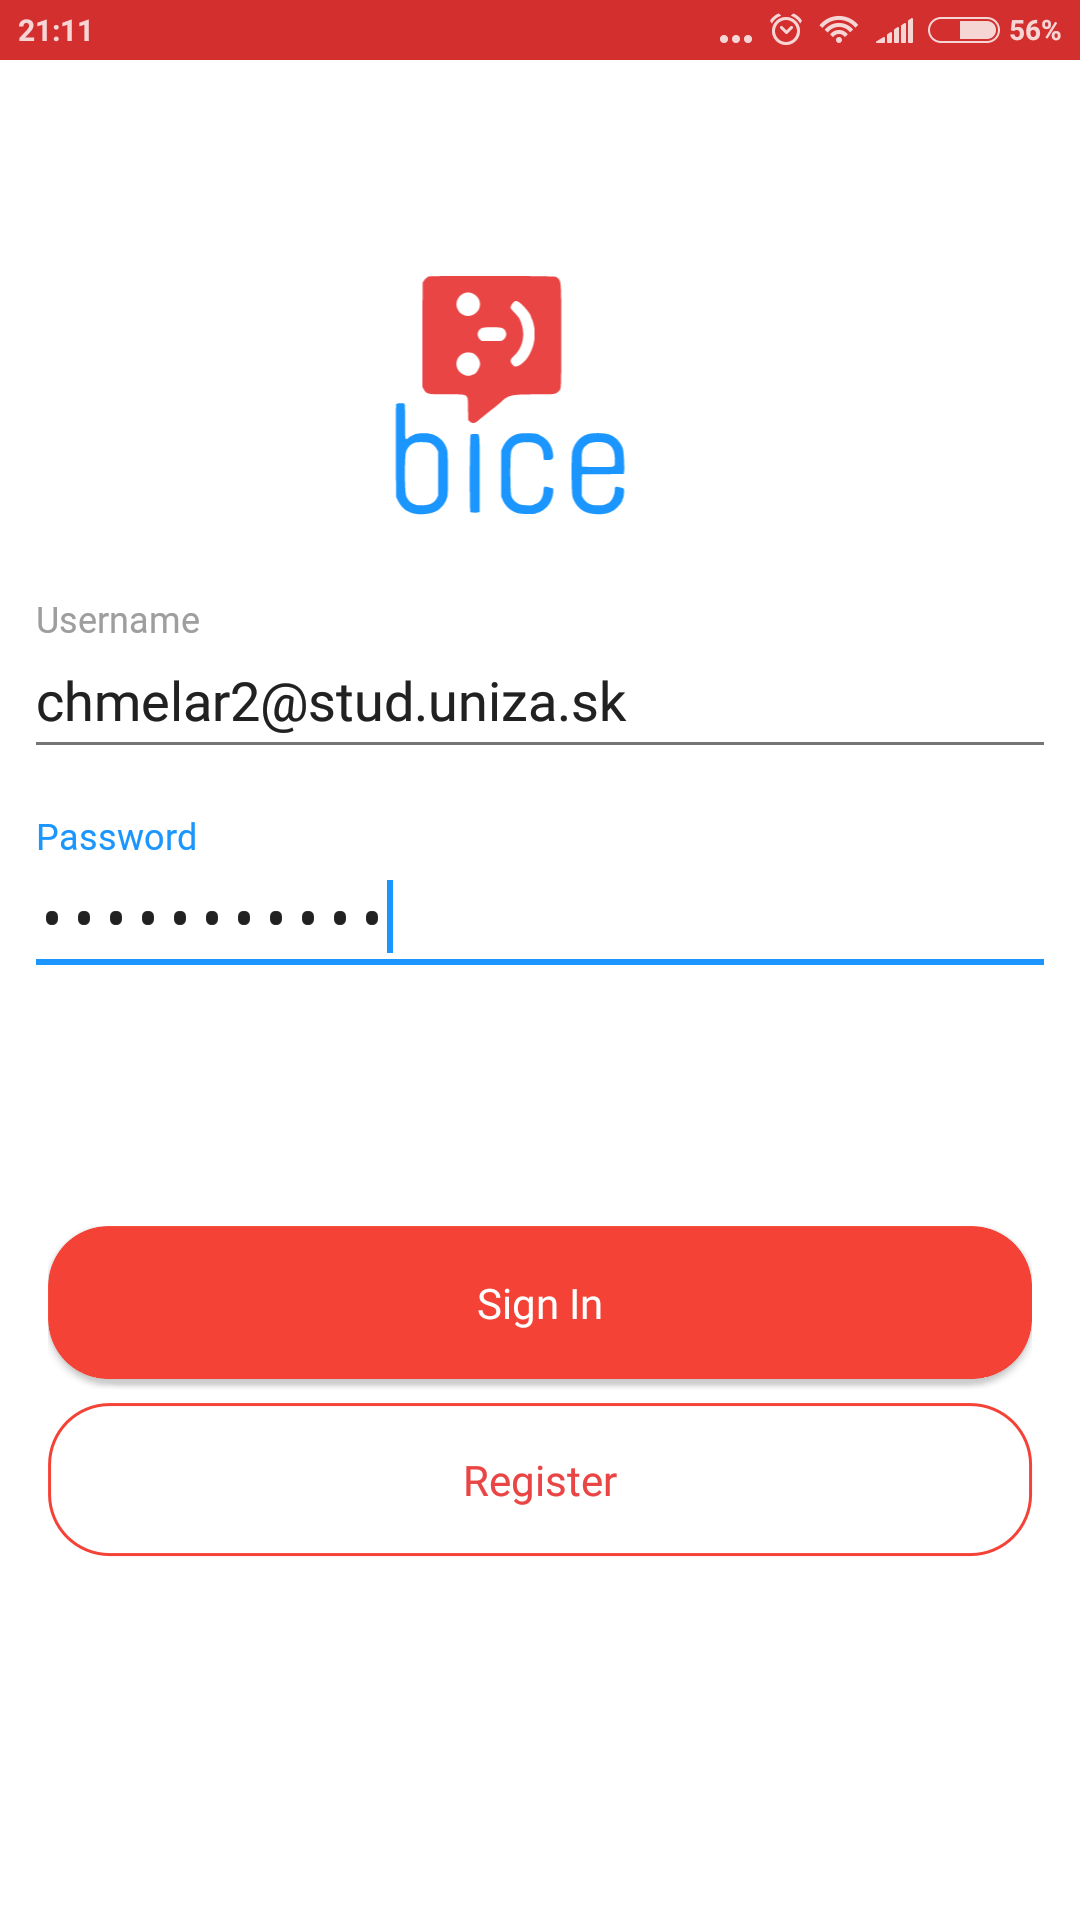
\includegraphics[width=0.7\textwidth]{images/login_screen.png} }
                \caption{Obrazovka prihlásenia}
                \label{obr3.3}
            \end{center}
        \end{minipage}
    \end{center}
\end{figure}




Pri inicializácii obrazovky vytvoríme inštanciu prezentéra, ktorý ako parametre akceptuje objekt typu \textit{IApiRoutes} na komunikáciu so serverom, a rozhranie \textit{IProjectsView}. Objekt \textit{IApiRoutes}  je vložený do prezentéra z hlavnej triedy \textit{App}. Trieda \textit{ProjectsActivity} implemetuje rozhranie \textit{IProjectsView} prezentéra, môže spracovať všetky správy odoslané prezentérom prostredníctvom rozhrania.

Po zadaní platnej adresy, ktorá je overovaná regulárnym výrazom, a heslom sa po stlačení červeného tlačítka na prihlásenie  zavolá metóda prezentéra, ktorá vola POST požiadavku, ktorej telo obsahuje JSON objekt s menom a heslom.

\vspace{10pt}
\begin{figure}[H]

    \begin{center}
        \begin{minipage}{1\linewidth}
            \begin{center}
               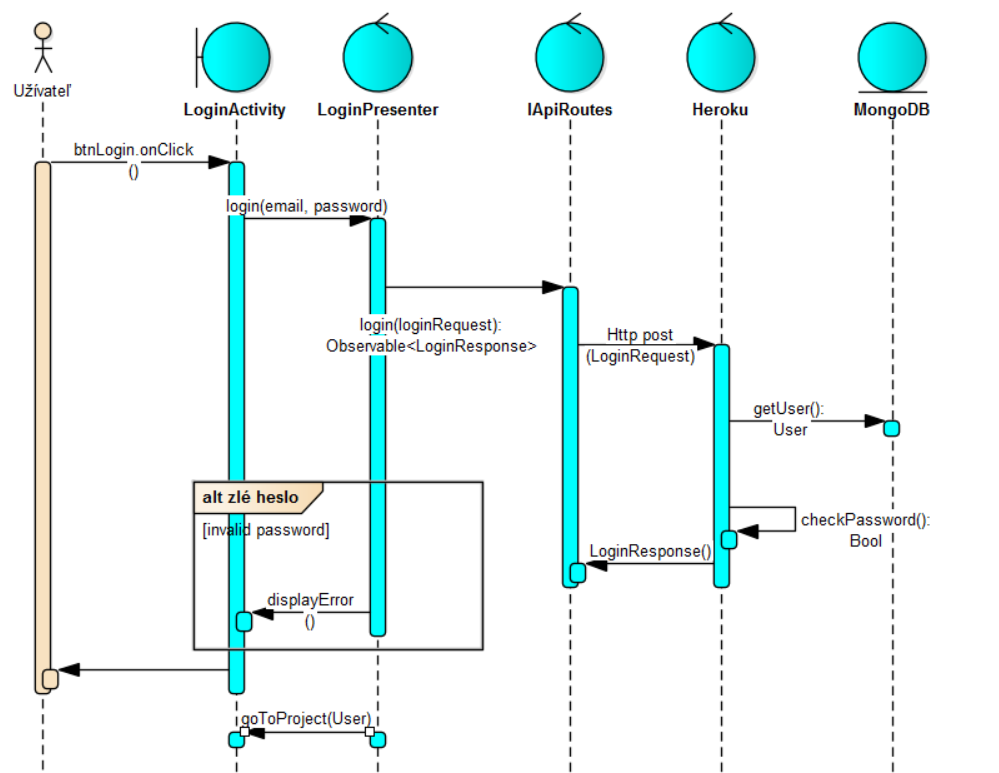
\includegraphics[width=1\textwidth]{images/login_rest.png}]   
                \caption{Sekvenčný diagram - Prihlasovanie }
                \label{obr3.5}
            \end{center}
        \end{minipage}
    \end{center}
    
\end{figure}
\vspace{10pt}

Server následne vyhľadá používateľa s požadovanou emailovou adresou. Spracuje heslo z tela požiadavky a porovná ho s kryptovanou verziou hesla. Po úspešnom porovnaní odošle server odpoveď v podobe JSON objektu s dátami o prihlásenom užívateľovi a \textit{JWT} kľúčom, ktorým sa môžeme identifikovať na serveri po dobu 24 hodín. Kľuč sa vkladá do Http klienta, ktorý ho automaticky vloží do hlavičky nasledujúcich požiadaviek.

\section{Obrazovka projektov}
Prihlasovacia obrazovka odoslala identifikačné číslo všetkých projektov, ktoré má používateľ zapísané. Prezentér odošle požiadavku na koncový bod servera \textit{/projects/:id}, kde \textit{:id} nahradí číslo projektu. Postupne sa projekty zobrazia na hlavnej obrazovke (obr.\ref{obr3.6}), odkiaľ používateľ pristupuje ku konkrétnym projektom.

\vspace{10pt}
\begin{figure}[H]

    \begin{center}
        \begin{minipage}{0.7\linewidth}
            \begin{center}
               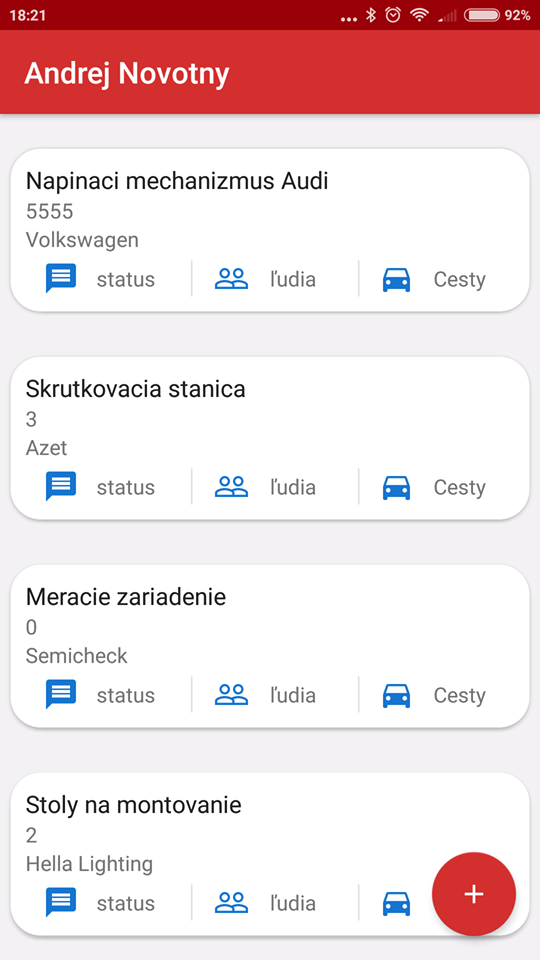
\includegraphics[width=0.7\textwidth]{images/screenz/main_screen.png}]   
                \caption{Obrazovka projektov}
                \label{obr3.6}
            \end{center}
        \end{minipage}
    \end{center}
    
\end{figure}
\vspace{10pt}


Po kliknutí na červené tlačítko so znakom ``+'' nás aplikácia presunie na obrazovku vytvorenia projektu (obr.\ref{obr3.7}).Obsahuje polia s nápovedou a automatickým dopĺňaním zamestnancov. Po vyplnení  požadovaných textových polí  odošle prezentér POST požiadavku na koncový bod  \textit{/projects/:id} s objektom JSON, ktorý obsahuje vyplnené dáta a čísla zamestnancov, ktorí budú pridaní do projektu. Následne sme presunutý na predošlú obrazovku. Aplikácia nás informuje o stave požiadavky \textit{toast} notifikáciou. 

\vspace{10pt}
\begin{figure}[H]

    \begin{center}
        \begin{minipage}{0.7\linewidth}
            \begin{center}
               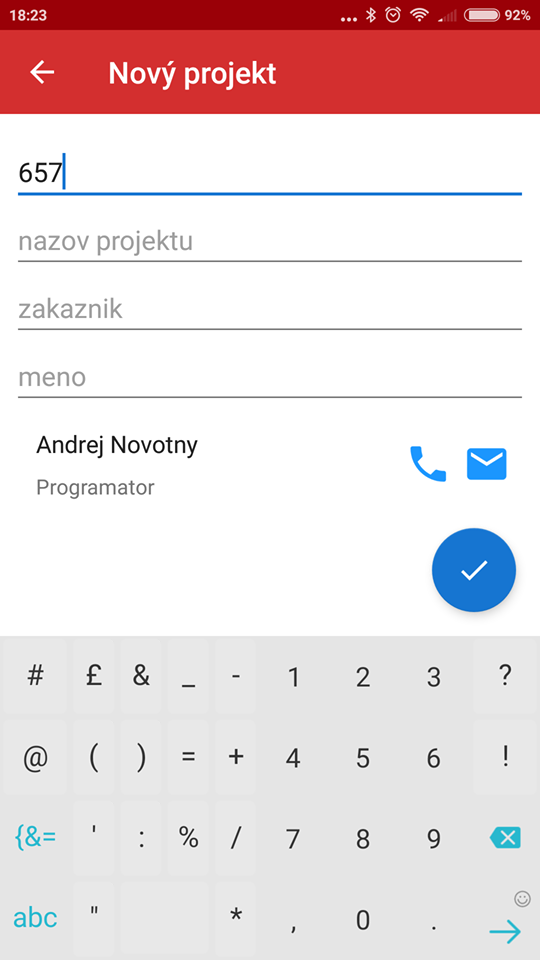
\includegraphics[width=0.7\textwidth]{images/screenz/projekt_new.png}]   
                \caption{Obrazovka vytvorenia projektu}
                \label{obr3.7}
            \end{center}
        \end{minipage}
    \end{center}
    
\end{figure}
\vspace{10pt}
 
\section{Detail projektov}

Detail obsahuje tri sekcie, medzi ktorými sa môžeme pohybovať kliknutím na prislúchajúcu záložku alebo potiahnutím prsta. Táto časť aplikácie je naprogramovaná v jazyku Kotlin. Obsahuje viacero komponentov ktoré sú veľmi podobné, ale s odlišnou logikou. Vďaka vlastnosti jazyka, ktorá umožňuje posielať funkciu ako parameter sme mohli znova použiť existujúce komponenty.

\subsection{Stav}

Zobrazuje posledné správy ktoré boli odoslané riešiteľmi projektu. Umožňuje odoslať aktualizáciu stavu prostredníctvom poľa v dolnej časti obrazovky. Podobne ako v predchádzajúcich obrazovkách, prezentér odosiela POST požiadavku na koncový bod  \textit{/projects/:id/comments} s textom komentára, číslom projektu a číslom užívateľa. Úspešné aktualizovaný stav sa zobrazí v zozname s časom odoslania a menom autora.

\vspace{10pt}
\begin{figure}[H]

    \begin{center}
        \begin{minipage}{0.7\linewidth}
            \begin{center}
               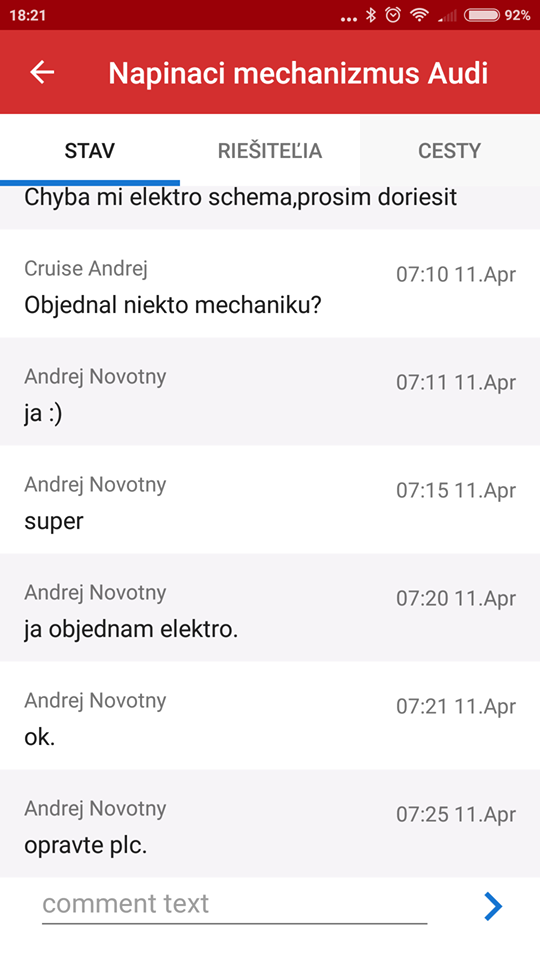
\includegraphics[width=0.7\textwidth]{images/screenz/stavy.png}]   
                \caption{Obrazovka stavov}
                \label{obr3.8}
            \end{center}
        \end{minipage}
    \end{center}
    
\end{figure}
\vspace{10pt}
\pagebreak
\subsection{Riešitelia}

V tejto záložke je vidieť všetkých používateľov, ktorí boli pridaní do projektu (obr.\ref{obr3.9}). Pri mene používateľa je zobrazená jeho pracovná pozícia, možnosť odoslať email alebo uskutočniť hovor. V spodnej časti obrazovky je možné pridať používateľa do projektu, alebo zorganizovať pracovné stretnutie. Kliknutím na ikonu pracovného stretnutia sa zobrazí dialóg na výber dátumu a času. Následne je používateľ presunutý na obrazovku s pred-vyplneným emailom na odoslanie (obr.\ref{obr3.10}). Email je adresovaný všetkým riešiteľom projektu.

\vspace{10pt}
\begin{figure}[H]

    \begin{center}
        \begin{minipage}{0.7\linewidth}
            \begin{center}
               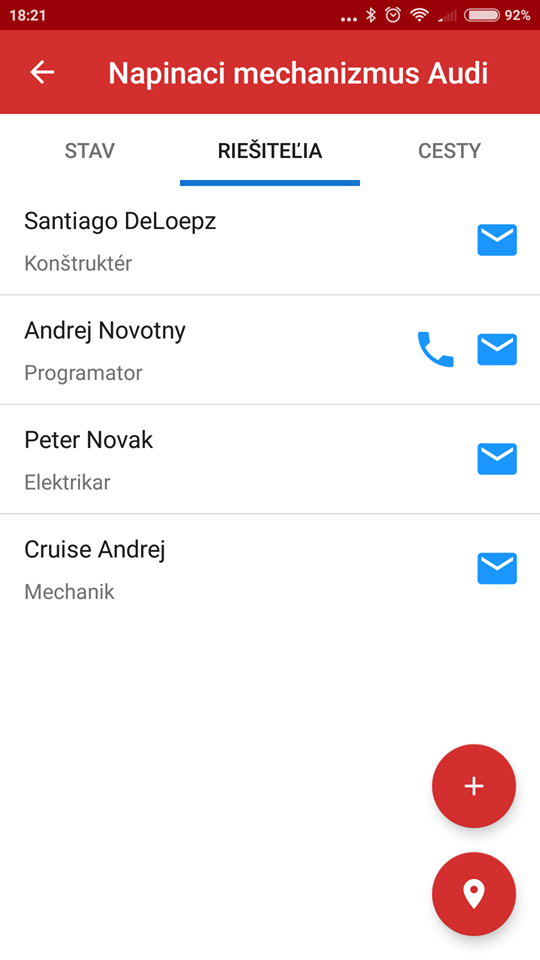
\includegraphics[width=0.7\textwidth]{images/screenz/riesitelia.png}]   
                \caption{Obrazovka riešiteľov}
                \label{obr3.9}
            \end{center}
        \end{minipage}
    \end{center}
    
\end{figure}
\vspace{10pt}

Výber emailového klienta je prenechaný na používateľa. Môže teda použiť akýkoľvek klient podľa vlastných preferencií

\vspace{10pt}
\begin{figure}[H]
  \centering
  \subfloat[Výber času stretnutia]{
    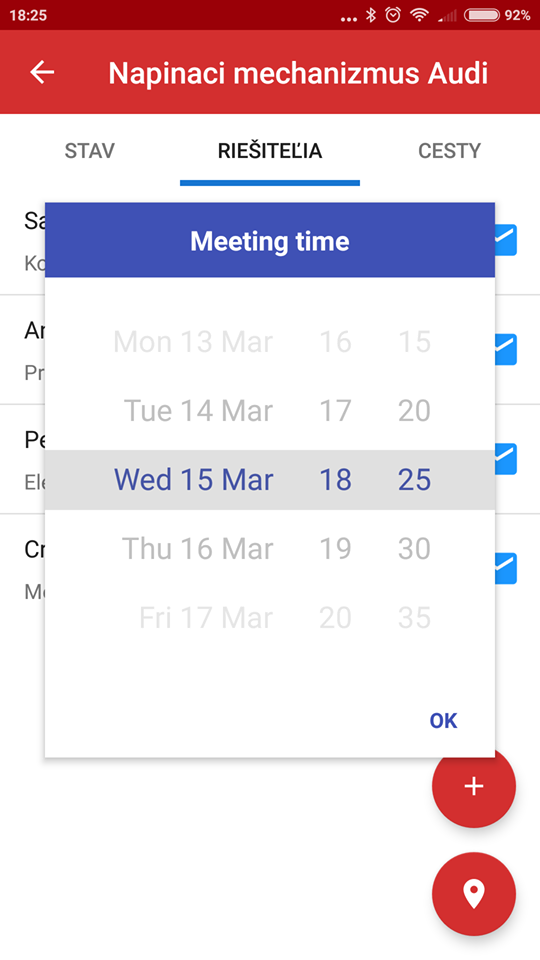
\includegraphics[width=0.4\textwidth]{images/screenz/meeting_datepicker.png}\label{obr3.11}
  }
  \hfill
  \subfloat[Pred-vyplnený email]{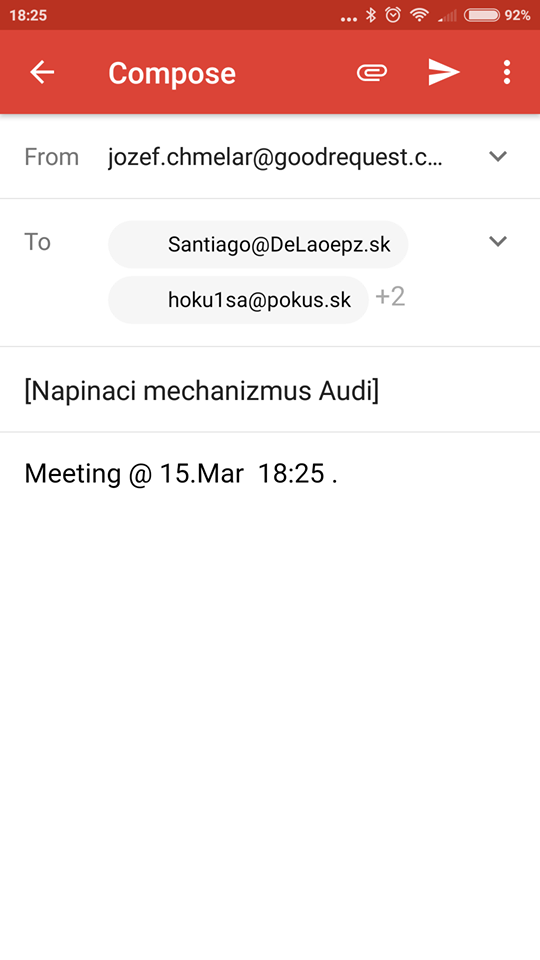
\includegraphics[width=0.4\textwidth]{images/screenz/meeting_mail.png}\label{obr3.10}}
    \caption{Obrazovky stretnutia}

\end{figure}

\subsection{Služobné cesty}
Obrazovka ktorá poskytuje prehľad všetkých pracovných ciest, s dôvodom cesty, autom a dátumom. Po kliknutí na špecifickú cestu sa zobrazí detail so zúčastnenými osobami. Po kliknutí na tlačítko s logom auta sme presmerovaný na obrazovku ktorá umožňuje pridanie novej cesty. Tu využijeme polia s automatickým dopĺňaním textu, a dialógu na výber dátumu
\vspace{10pt}
\begin{figure}[H]
  \centering
  \subfloat[Prehľad služobných ciest]{
    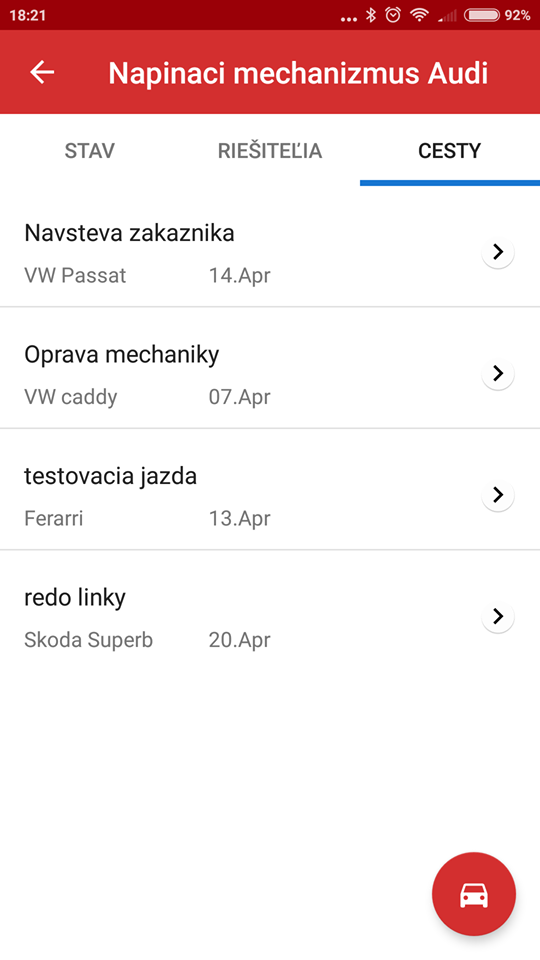
\includegraphics[width=0.4\textwidth]{images/screenz/cesty.png}\label{obr3.11}
  }
  \hfill
  \subfloat[Pred-vyplnený email]{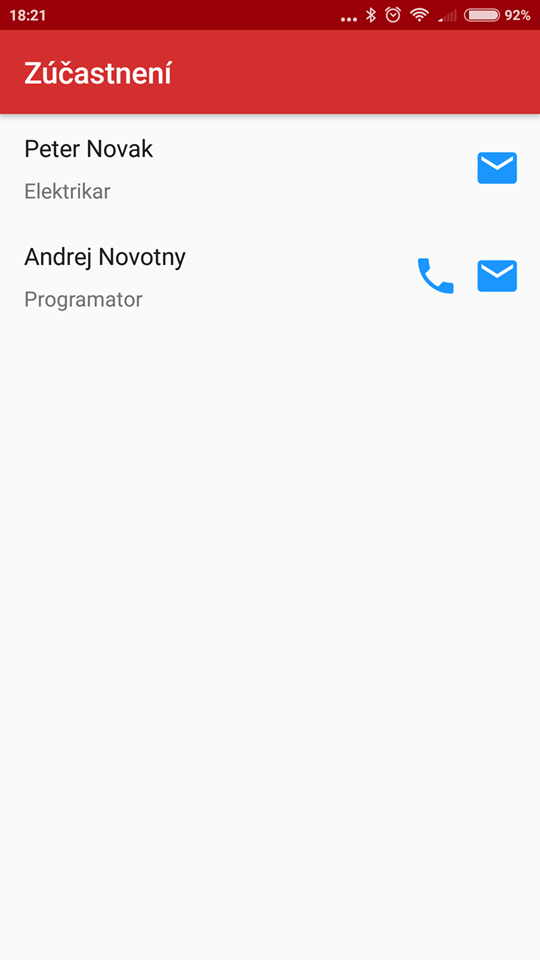
\includegraphics[width=0.4\textwidth]{images/screenz/cesty_zucastneni.png}\label{obr3.10}}
    \caption{Detail služobnej cesty}
\end{figure}

\vspace{10pt}

\section{Serverová časť}

Aplikácia musí fungovať z akejkoľvek siete bez nutnosti využívať VPN (virtual private network) na prístup do firemnej siete, rozhodli sme sa teda pre využitie zadarmo prístupných služieb \textit{Heroku}  ktoré poskytuje hosting pre NodeJS aplikáciu, ktorá je naprogramovaná použitím frameworku ExpressJS, ktorý uľahčuje prácu pri vytvárani REST API. Aplikácia je napojená na databázu ktorú poskytuje server \textit{Mlab.com}. Jedná sa o bezplatnú inštanciu  noSQL databázy MongoDB. MongoDB je vhodný nástroj, pretože na komunikáciu medzi zariadeniami používame formát JSON, ktorý je prirodzený pre Mongo,Node.JS a najpoužívanejší pre REST API. API poskytuje koncové body na vytváranie, editovanie, mazanie a získavanie dát z databázy.

\subsection{Bezpečnosť}

Dôležitou súčasťou každej aplikácie je bezpečnosť a zamedzenie prístupu neoprávneným osobám k citlivým dátam. Framework s ktorým pracujem, \textit{Express.JS}, poskytuje funkciu zvanú ``middleware''\cite{express}, ktorá umožňuje narušiť cyklus požiadavky. Pri každej požiadavke na server sa spustí práve táto funkcia, ktorá hľadá v hlavičke požiadavky kľúč \textit{x-access-token}. Ak je dekódovaný kľuč platný, funkcia zavolá metódu \textit{next()}, ktorá spustí požadovaný proces. Pokiaľ kľúč nie je platný, server odpovie Http kódom 403, prístup zamietnutý. 

Pri vytvorení nového používateľa sa do databázy ukladá zakódovaná verzia jeho hesla. Hash hesla je generovaný pomocou knižnice JWT a bcrypt. Každé heslo je ``osolené'' náhodným a tajným reťazcom znakov, ktorý je uložený ako premenná prostredia na Heroku. Pokiaľ majú dvaja užívatelia rovnaké heslo, nie sme to schopní zisiť pri pohľade na tabuľku užívateľov v databáze, keďže sú uložené ako úplne odlišné 60 znakové reťazce.

\subsection{Databáza}

Ako databázový systém bol zvolená  noSQL databáza MongoDB, ktorej inštanciu nám poskytuje služba mLab. Aplikácia sa po spustení na serveri okamžite pripája k databázovej URL, ktorá je  uložená na Heroku v premenných prostredia, pretože obsahuje meno a heslo potrebné k pripojeniu. Následne komunikujeme s databázou pomocou \textit{ORM Mongoose}. \textit{ORM} automaticky mení odpoveď databázy na objekt, vyhľadáva, filtruje a automaticky spája tabuľky pomocou cudzieho kľúča. MongoDB nie je relačná databáza, označuje sa termínom noSQL  - ``not only SQL''. Nie je viazaná modelom a môže byť kedykoľvek zmenená, nezaručuje teda konzistentnosť dát. Preto používame objekty typu \textit{commentSchema}. V schéme  definujeme štruktúru dát a referencie na ostatné tabuľky.
\vspace{10pt}

\begin{lstlisting}[language=JavaScript]
var commentSchema = new Schema({	
    author: {type: Number , ref:'Employee', required: true},
    text: { type: String, required: true },    
    createdAt: {type: Date,  default: Date.now}
}
\end{lstlisting}

Ako príklad, použijeme najjednoduchšiu schému \textit{commentSchema}. Obsahuje referenciu na tabuľku \textit{Employee} s rovnakým typom ako je primárny kľúč v odkazovanej tabuľke. Automaticky je vytvorená aj premenná \textit{objectId}, ktorá je jednoznačným identifikátorom  pre \textit{commentSchema}. 
\vspace{10pt}


\begin{figure}[H]
    \begin{center}
        \begin{minipage}{0.7\linewidth}
            \begin{center}
     \frame{            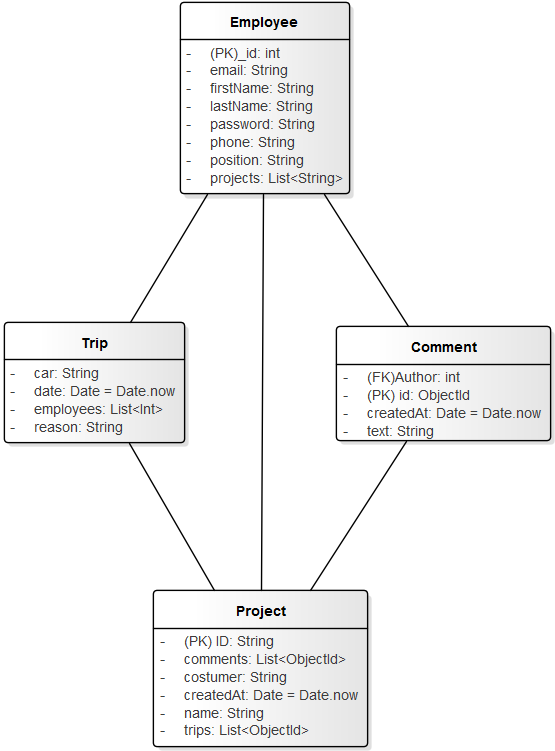
\includegraphics[width=1\textwidth]{images/dbModel.png} }
                \caption{Model databázy}
                \label{obr4.12}
            \end{center}
        \end{minipage}
    \end{center}
\end{figure}



\chapter*{Záver}
\addcontentsline{toc}{chapter}{Záver}

Bakalárska práca sa zaoberá vývojom aplikácie pre Android, ktorá by uľahčila organizáciu práce projektovému manažérovi. Sprehľadnila stav projektu, zjednotila ľudí pracujúcich na projekte pod spoločné rozhranie, ktoré na komunikáciu využíva stále používaný email, obyčajné telefonáty a stav projektu ktorý už nie je zakopaný v nekonečnej spleti emailov.

Celá práca bola navrhnutá tak, aby sa do budúcnosti ľahko implementovalo webové, alebo ďalšie mobilné rozhranie, nové funkcie a kvôli rozšíriteľnosti databázy, ďalšie dáta o projekte, prípadne používateľoch. 

Pri vypracovávaní práce sme získali veľké množstvo skúseností. Vďaka analýze sme si mohli prezrieť veľké množstvo frameworkov, databáz, architektonických vzorov pre vývoj aplikácií a posledných     technológií. Z veľkého výberu programovacích jazykov a vzorov sme si vybrali tie najjednoduchšie a najintuitívnejšie, aby  výsledkom našej práce bol čistý a  prehľadný kód s minimálnym technologickým dlhom.

Prišli sme k záveru, že aj zdanlivo jednoducho znejúce zadanie si na vypracovanie vyžaduje veľa času, prehľad v technológiách a trpezlivosť. Vypracovali sme aplikáciu, ktorá funguje na rovnakom princípe ako väčšina najpoužívanejších aplikácii ako sú napríklad Facebook, preto máme do budúcnosti vzácne skúsenosti ohľadom vývoja mobilných aplikácií, ktoré sú zo dňa na deň žiadanejšie. 

Do aplikácie by sme v budúcnosti radi implementovali pridelenie požiadavky konkrétnemu riešiteľovi s notifikáciou o blížiacom sa konečnom termíne a webové rozhranie, ktoré bude už vďaka hotovej serverovej časti rýchlejšie implementované. Ďalej službu monitorujúcu aktivitu používateľov na všetkých obrazovkách a získavanie údajov o chybách pomocou služby \textit{Crashlytics}. Aplikácia je ľahko rozšíriteľná, a preto sa vieme rýchlo prispôsobiť požiadavkám firmy o ďalšiu funkcionalitu.

%%%%%%%%%%%%%%%%%% bilbiografia

%%%%%%%%%%%%%%%%%%%%%%%%%%%%%%%%%%%%%%%%%%%%%%%%%%%%%%%%%%%%%%%%%%%%%%%%%%%%%
\begin{thebibliography}{99}                                
\label{literatura}
%\addcontentsline{toc}{section}{Literatúra}
% \addcontentsline{toc}{chapter}{Literatúra}

\bibitem{android}
Android, \textit{Android - Android is for everyone} [online], [Marec,2017], Dostupné na internete:  \url{android.com/everyone/enabling-opportunity/}

\bibitem{cena_smartphone}
bcg.perspectives, \textit{The Growth of the Global Mobile Internet Economy} [online], [Marec,2017], Dostupné na internete:\url{bcgperspectives.com/content/articles/telecommunications_connected_world_growth_global_mobile_internet_economy/}


\bibitem{pocetTelefonov}
OpenSignal, \textit{Android Fragmentation Visualized} [online], [Marec,2017], Dostupné na internete: \url{opensignal.com/reports/2015/08/android-fragmentation/}


\bibitem{usage}
Dashboards, \textit{Home - Android - Dashboards} [online], [Marec,2017], Dostupné na internete: \url{developer.android.com/about/dashboards/index.html#Platform}

\bibitem{playstore_alt}
Digitaltrends, \textit{ Tired of Google Play?} [online], [Marec,2017], Dostupné na internete: \url{digitaltrends.com/mobile/android-app-stores/}

\bibitem{history_cameras}
Verge, \textit{ Before it took over smartphones, Android was originally destined for cameras} [online], [Marec,2017], Dostupné na internete: \url{theverge.com/2013/4/16/4230468/}


\bibitem{history_android}
PhoneArena, \textit{ Google's Android OS: Past, Present, and Future} [online], [Marec,2017], Dostupné na internete: \url{phonearena.com/news/Googles-Android-OS-Past-Present-and-Future_id21273/}

\bibitem{versions}
Social Compare, \textit{Android versions comparison} [online], [Marec,2017], Dostupné na internete: 
\url{socialcompare.com/en/comparison/android-versions-comparison}

 
\bibitem{dalvik}
Engadget, \textit{'ART' experiment in Android} [online], [Marec,2017], Dostupné na internete: 
\url{engadget.com/2013/11/06/new-android-runtime-could-improve-battery-life/}

\bibitem{android_developers}
Android Developers, \textit{Activity} [online], [Marec,2017], Dostupné na internete: 
\url{developer.android.com/reference/android/app/Activity.html}

\bibitem{android_code}
OpenHub, \textit{The Android Open Source project on OpenHub} [online], [Marec,2017], Dostupné na internete: 
\url{openhub.net/p/android/analyses/latest/languages_summary}


\bibitem{ndkVsSdk}
Android Authority, \textit{Java vs C app performance} [online], [Marec,2017], Dostupné na internete: 
\url{androidauthority.com/java-vs-c-app-performance-689081/}

\bibitem{os_usage}
Quartz Media LLC, \textit{Android just hit a record 88\% market share of all smartphones} [online], [Marec,2017], Dostupné na internete: 
\url{qz.com/826672/android-goog-just-hit-a-record-88-market-share-of-all-smartphones/}


\bibitem{mvpdef}
Antonio Leiva \textit{MVP for Android: how to organize the presentation layer} [online], [Marec,2017], Dostupné na internete: 
\url{antonioleiva.com/mvp-android/}


\bibitem{androidstudio}
Android Developers Blog \textit{An update on Eclipse Android Developer Tools} [online], [Marec,2017], Dostupné na internete: 
\url{android-developers.googleblog.com/2015/06/an-update-on-eclipse-android-developer.html}

\bibitem{androidstudio2}
Stack tips
 \textit{Android Studio Features} [online], [Marec,2017], Dostupné na internete: 
\url{stacktips.com/tutorials/android/android-studio-features}

\bibitem{androidstudio3}
Idea blog \textit{IntelliJ IDEA and Android Studio FAQ} [online], [Marec,2017], Dostupné na internete: 
\url{blog.jetbrains.com/idea/2013/05/intellij-idea-and-android-studio-faq/}
 
 \bibitem{kotlin}
Mike Hearn \textit{Why Kotlin is my next programming language} [online], [Marec,2017], Dostupné na internete: 
\url{ medium.com/@octskyward/why-kotlin-is-my-next-programming-language-c25c001e26e3/}
 
  \bibitem{heroku}
crunchbase \textit{Heroku}[online], [Marec,2017], Dostupné na internete: 
\url{ crunchbase.com/organization/heroku#/entity}

  \bibitem{clientserver}
Business Dictionary
 \textit{What is client-server architecture?    }[online], [Marec,2017], Dostupné na internete: 
\url{www.businessdictionary.com/definition/client-server-architecture.html }


  \bibitem{express}
Express
 \textit{Using Express middleware}[online], [Marec,2017], Dostupné na internete: 
\url{expressjs.com/en/guide/using-middleware.html }
 
% Autor. Názov : podnázov (nepovinný). Poradie vydania. Miesto vydania: vydavateľ, rok vydania. Rozsah strán. ISBN

% \bibitem{cocoa_touch}
% Kelley Jeff,
% {\it Learn Cocoa Touch for iOS}, New York, Springer Science+Business Media 2012, ISBN 978-1-4302-4269-7.

\end{thebibliography}	%  Bilbiografia

\end{document}

